\documentclass[11pt,a4paper]{article}
\usepackage{fontspec}
\setmainfont{TeX Gyre Pagella}
\newfontfamily\headfont{Inter}[UprightFont=*-ExtraBold,BoldFont=*-ExtraBold,Extension=.otf,Path=/usr/share/fonts/opentype/inter/]
\usepackage[a4paper,margin=2.3cm]{geometry}
\usepackage{graphicx,booktabs,float,caption,array,xcolor,longtable}
\usepackage{xurl}
\usepackage[hidelinks]{hyperref}
\usepackage{titlesec}
\usepackage[round]{natbib}
\usepackage{setspace}
\setstretch{1.05}
\renewcommand{\topfraction}{0.9}
\renewcommand{\bottomfraction}{0.8}
\renewcommand{\textfraction}{0.1}
\renewcommand{\floatpagefraction}{0.75}
\setlength{\parindent}{0pt}
\setlength{\parskip}{0.55em}
\titleformat{\section}{\headfont\Large}{\thesection}{0.8em}{}
\titleformat{\subsection}{\headfont\large}{\thesubsection}{0.8em}{}
\captionsetup{font=small,labelfont=bf}
\urlstyle{same}
\hypersetup{pdftitle={Ancient DNA on the Map},pdfauthor={Tristan Hotham}}

\begin{document}
\begin{center}
{\Large\bfseries Ancient DNA on the Map\par}
\vspace{0.4em}
{\large Where and when the world's published ancient human genomes lived:\\16,496 individuals in the Allen Ancient DNA Resource\par}
\vspace{1.2em}
{\large Tristan Hotham\par}
\vspace{0.3em}
{\small Independent researcher\\
ORCID: 0000-0003-4931-9349\\
DOI: https://doi.org/10.5281/zenodo.23872993\par}
\vspace{0.8em}
2026
\end{center}

\begin{quote}
\small
\begin{center}\textbf{Abstract}\end{center}
I place every ancient individual in the Allen Ancient DNA Resource (AADR), release v66.p1, on a map by burial place and date, and use the archive's own annotations to describe its coverage and two well known episodes of European prehistory. Of 17,629 ancient individuals, 16,496 (94\%) have at least one data set that passes the archive's quality assessment. They come from 3,664 sites in 127 present-day countries and span 43,925 BCE to 1890 CE, though half lived after 450 BCE; 80\% were first published in 2020 or later. Sampling is heavily skewed: 68.4\% of located modern humans were buried in Europe, which holds 9.2\% of today's population and 7.5\% of the land, while Africa supplies 1.9\% for 17.1\% of the population. The earliest individuals labelled Neolithic in each of 24 countries of Europe and Anatolia become later with distance from central Anatolia, by 0.88 years per kilometre (r = 0.75), an apparent spread of about 1.1 km a year. Y chromosome haplogroups, used here as a proxy for male lines and not for ancestry, change abruptly around 2500 BCE: in Britain none of 76 men dated before 2500 BCE carries R1b, against 50 of 56 (89.3\%) from 2500 to 1500 BCE, and in Iberia, Scandinavia and central Europe R1b and R1a together rise from under 5\% of men before 3000 BCE to at least half after 2500 BCE.

\textbf{Keywords:} ancient DNA; archaeogenetics; Y chromosome; mitochondrial DNA; Neolithic; Bell Beaker; Yamnaya; sampling bias; open data; mapping
\end{quote}

\section{Introduction}
Since the first ancient human genome was published in 2010, ancient DNA has reshaped the study of the human past. Thousands of individuals have now been sequenced, and the Allen Ancient DNA Resource \citep{aadr,aadrpaper} gathers the published data in one curated, openly licensed release, with an annotation file that records for each individual its date, place, archaeological group, genetic sex, uniparental haplogroups and a quality assessment.

This paper does three simple things with that annotation file. First, it describes the archive as a whole: how many individuals, from when and where, and how the sample relates to the world's population and land. Second, it asks whether the earliest individuals labelled Neolithic in each country show the familiar spread of farming out of Anatolia. Third, it tracks Y chromosome haplogroups R1b and R1a through time in four regions of Europe, as a simple proxy for the arrival of male lines associated with steppe populations in the third millennium BCE. None of these uses genome-wide ancestry, which the original studies measure; everything here can be checked against the annotation file alone. The paper accompanies an interactive map (\url{https://maps.tristanhotham.com/ancient-dna/}).

\section{Data}
The AADR release v66.p1 public 1240K annotation file has 23,089 rows, one for each data representation of an individual. 3,970 rows describe present-day people (date 0 before present) and 19,118 describe 17,629 ancient individuals; 1,489 rows are additional representations of an individual already counted. The columns used are the Individual ID, the date mean and standard deviation in years before 1950 (BP) with the full date description, the Group ID, locality, political entity, latitude and longitude, the number of SNPs hit on the 1240k set, molecular sex, the automatic ISOGG Y haplogroup and the manual Y call where one is given, the mtDNA haplogroup, the first publication and the ASSESSMENT field. Present-day population and land area come from Natural Earth \citep{naturalearth}.

\begin{table}[tbp]\centering\small\caption{The twenty present-day countries and territories with the most ancient individuals passing the quality assessment.}\label{tab:countries}\begin{tabular}{lrr}\toprule Country or territory & Individuals & Share\\\midrule
Russia & 1,394 & 8.4\%\\
Hungary & 1,317 & 8.0\%\\
United Kingdom & 1,151 & 7.0\%\\
China & 865 & 5.2\%\\
Austria & 784 & 4.8\%\\
Italy & 698 & 4.2\%\\
Denmark & 653 & 4.0\%\\
Germany & 617 & 3.7\%\\
Spain & 594 & 3.6\%\\
France & 537 & 3.3\%\\
Turkey & 476 & 2.9\%\\
Belgium & 453 & 2.8\%\\
Czechia & 452 & 2.7\%\\
Poland & 437 & 2.6\%\\
Sweden & 374 & 2.3\%\\
Ukraine & 325 & 2.0\%\\
Croatia & 270 & 1.6\%\\
Mongolia & 264 & 1.6\%\\
Argentina & 258 & 1.6\%\\
Kazakhstan & 239 & 1.4\%\\
\bottomrule\end{tabular}\end{table}

\section{Methods}
\subsection{Individuals and quality}
A row passes if its ASSESSMENT begins with \texttt{Pass}, \texttt{PROVISIONAL\_PASS} or \texttt{MERGE\_PASS}. An individual is kept if at least one of its rows passes, and is represented by the passing row with the most SNPs. This keeps 16,496 individuals (14,850 Pass, 1,577 provisional, 69 merged); the stricter rule of taking each individual's richest row and then filtering keeps 16,267. The 1,133 individuals with no passing row are excluded from all counts. 8 individuals whose Group ID names Neanderthals or Denisova Cave and whose date is older than 40,000 BP are treated as archaic humans and excluded from the analyses of modern humans. 88 kept individuals lack coordinates.

\subsection{Dates, labels and haplogroups}
Calendar years are 1950 minus the date mean. Each individual is given a broad period from its date and a culture label from words in its Group ID (for example \texttt{N} or \texttt{EN} for Neolithic, \texttt{BA} for Bronze Age, \texttt{BellBeaker}, \texttt{CordedWare}, \texttt{Yamnaya}), with named cultures taking priority over periods; the rules are listed in the code. Y haplogroups are grouped by their leading characters into major clades (R1b, R1a, I1, I2, G2, J1, J2, E1b, and N, Q, C, O, H, T, L, D). Calls at a higher level than these (such as CT, F, K, P, R or R1) cannot distinguish R1a from R1b and are excluded from shares; of 8,599 men, 7,750 (90.1\%) have a resolved call. mtDNA haplogroups are grouped by their leading letter. Sex is the archive's molecular sex.

\subsection{Continents and sampling}
Each located individual is assigned to the Natural Earth country polygon that contains it, or the nearest within 150 km. Continents follow Natural Earth, except that Russia is split at 60°E. Shares of present-day population (2019 estimates; Russia's divided in proportion to the population of its towns on each side of 60°E, 73.2\% to the west) and of land area (equal-area projection, without Antarctica) are compared with the share of individuals.

\subsection{Neolithic arrival}
For Europe and Anatolia (latitude 30 to 72°N, longitude 12°W to 45°E), I take modern humans labelled Neolithic, leave out Russia, Ukraine, Belarus, Moldova, the Baltic states and Finland (where the label usually denotes pottery-using hunter-gatherers), groups whose labels also name hunter-gatherers (47 individuals), dates with a standard deviation over 300 years, and dates whose mean lies outside their own stated range. This leaves 1,597 individuals. For each country with at least three, the earliest by date mean marks the first sampled Neolithic burial, and its great circle distance from Çatalhöyük (37.67°N 32.83°E) is computed. A least squares line of date on distance is fitted without Turkey.

\subsection{Y lines through time}
Men with a resolved Y call are grouped into 500 year bins in four regions: Britain (England, Scotland and Wales), Iberia (Spain, Portugal and Gibraltar), Scandinavia (Denmark, Sweden and Norway) and central Europe (Germany, Czechia, Austria, Switzerland, Poland and Slovakia). The share carrying R1b or R1a is computed per bin; bins with fewer than five men are shown but not interpreted.

\section{Results}
\subsection{The archive}
Figure~\ref{fig:map} shows all 16,400 located modern humans. The oldest are dated to 43,925 BCE (Ranis, Germany, and Zlatý kůň, Czechia), and 102 lived before 10,000 BCE; 79.5\% lived after 3000 BCE (Figure~\ref{fig:archive}). The archaic genomes range back to 183,050 BCE (Denisova 25). Molecular sex is male for 8,601, female for 6,835 and unknown for 1,060 (1.26 men per woman). 3,757 individuals were first published in 2025, and 80.0\% in 2020 or later. The largest single source is PattersonReichNature2021 (741 individuals). 1,641 of 3,630 sites (45.2\%) contribute one individual; the most sampled are Avar period cemeteries in Austria and Hungary.

\begin{figure}[tbp]\centering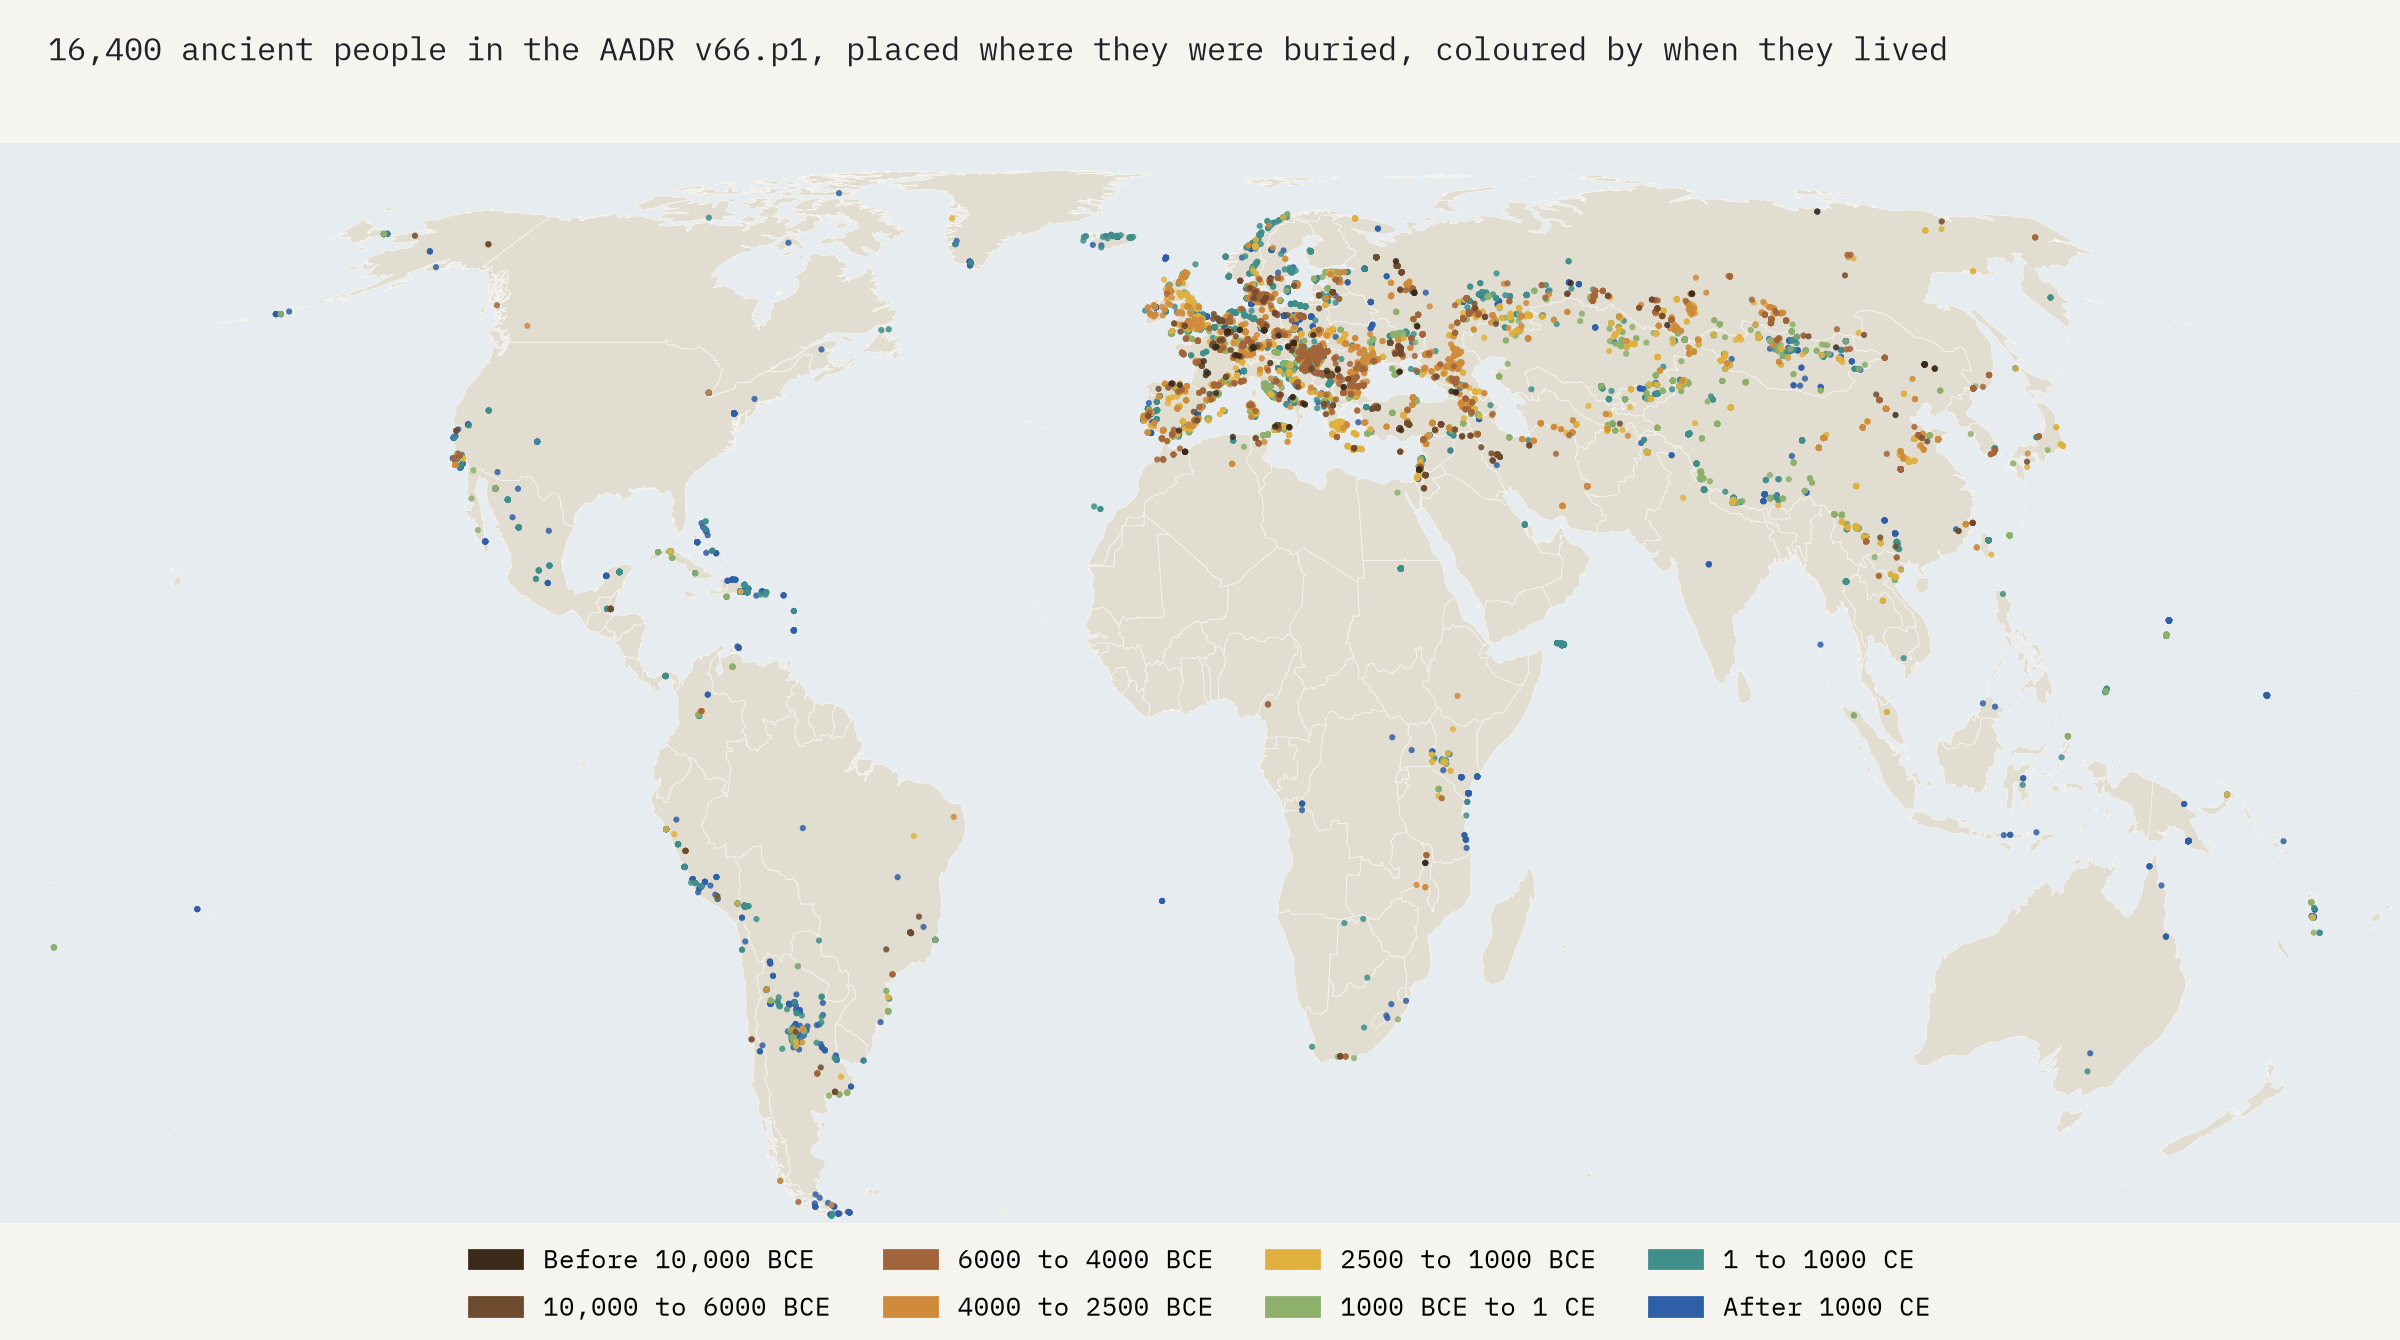
\includegraphics[width=\textwidth]{f_map.png}
\caption{Every located modern human in the AADR v66.p1 that passes the quality assessment, coloured by broad period.}\label{fig:map}\end{figure}

\begin{figure}[tbp]\centering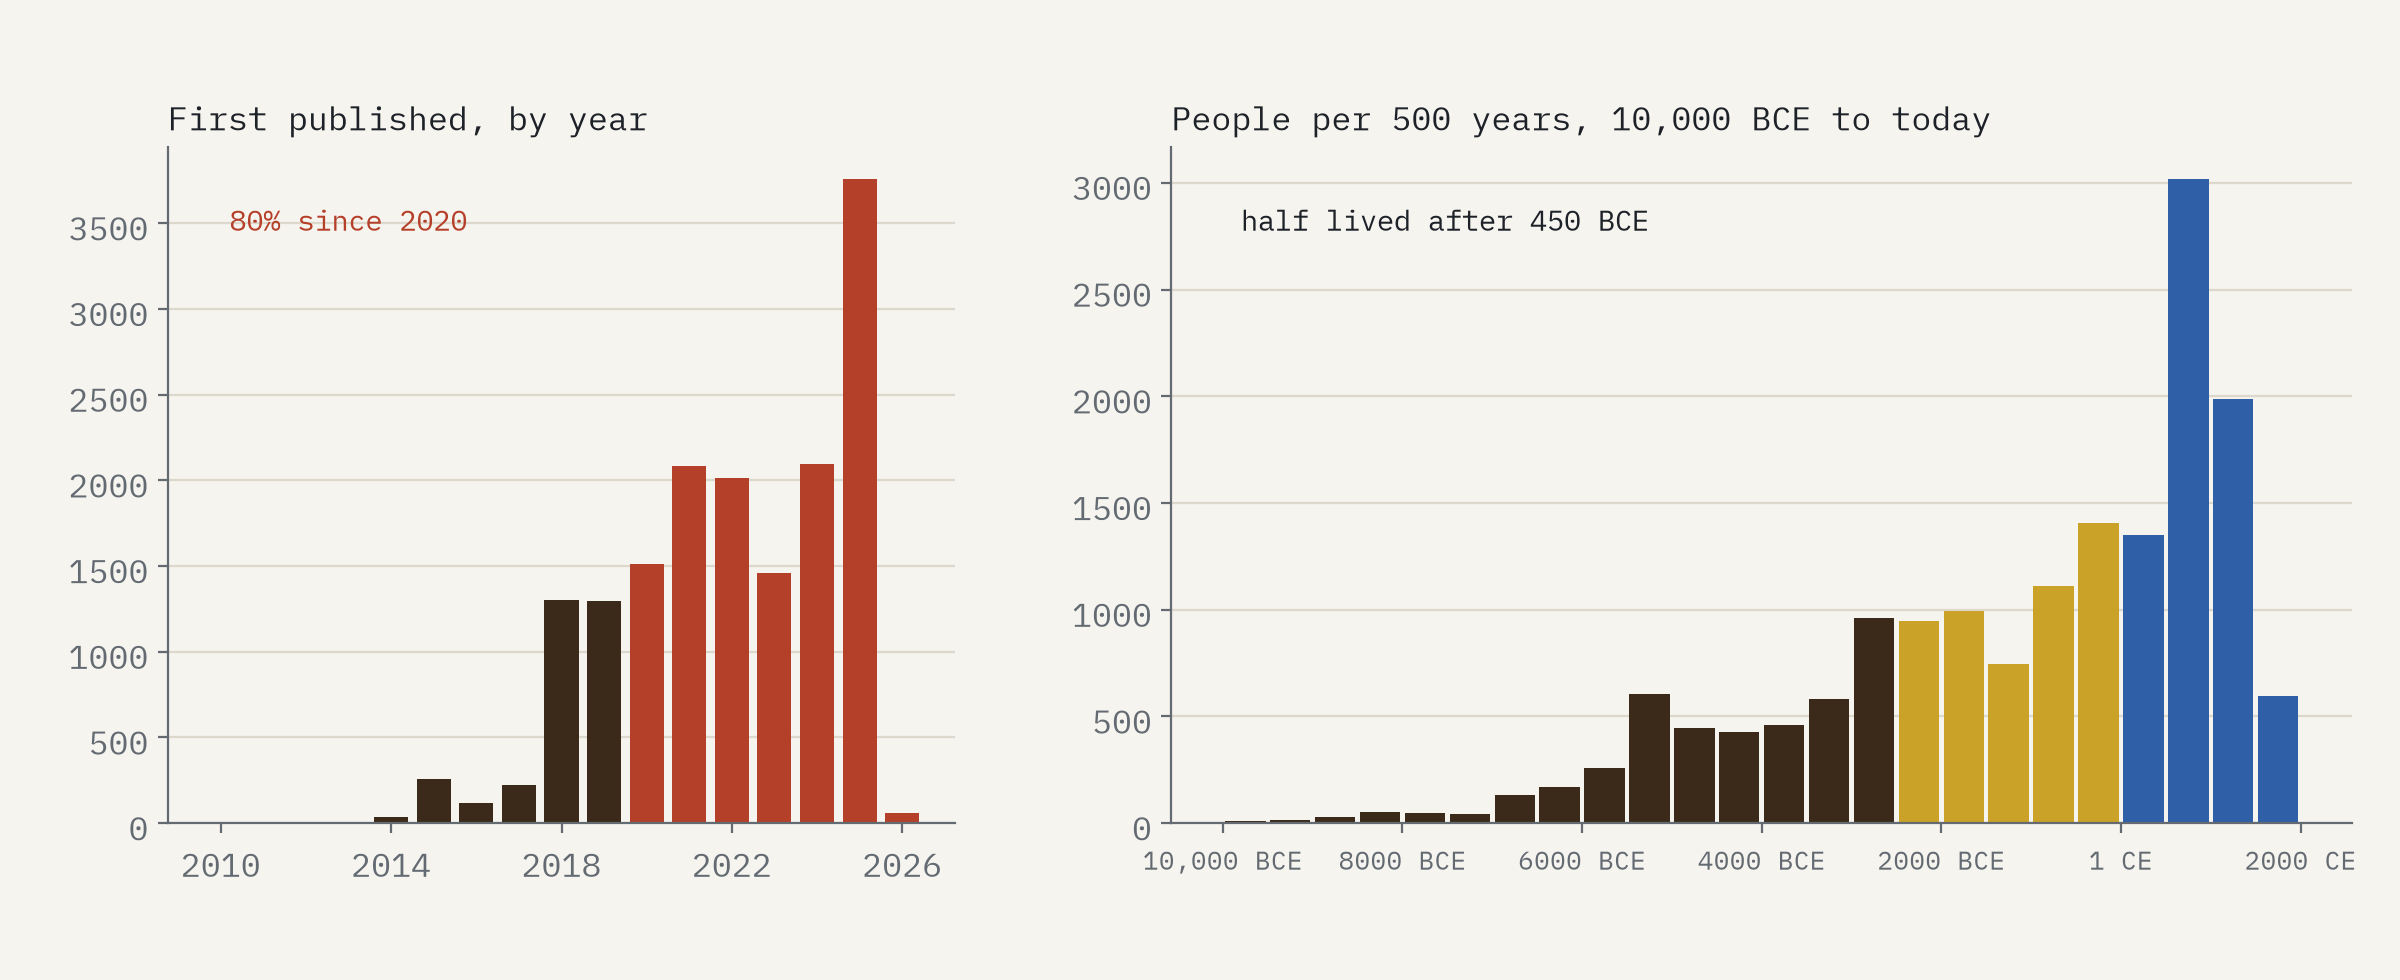
\includegraphics[width=\textwidth]{f_archive.png}
\caption{Left: individuals by year of first publication. Right: individuals per 500 years since 10,000 BCE.}\label{fig:archive}\end{figure}

\subsection{Sampling bias}
Europe supplies 11,217 of 16,400 located individuals (68.4\%), 7.4 times its share of present-day population and 9.2 times its share of land (Table~\ref{tab:bias}, Figure~\ref{fig:bias}). Asia supplies 21.8\% for 60.0\% of the population, Africa 1.9\% for 17.1\%. Per head of present-day population Europe has about 66 times as many ancient genomes as Africa. Europe's share exceeds half in seven of the eight broad periods; the exception is 10,000 to 6000 BCE (41.6\%).

\begin{table}[tbp]\centering\small\caption{Located modern humans by continent, against present-day population and land.}\label{tab:bias}\begin{tabular}{lrrrrr}\toprule Continent & Individuals & Share & Population & Land & Per 10 million people\\\midrule
Europe & 11,217 & 68.4\% & 9.2\% & 7.5\% & 158.5\\
Asia & 3,571 & 21.8\% & 60.0\% & 32.8\% & 7.8\\
Africa & 308 & 1.9\% & 17.1\% & 22.2\% & 2.4\\
North America & 595 & 3.6\% & 7.6\% & 18.1\% & 10.2\\
South America & 449 & 2.7\% & 5.6\% & 13.1\% & 10.5\\
Oceania & 260 & 1.6\% & 0.6\% & 6.3\% & 61.3\\
\bottomrule\end{tabular}\end{table}

\begin{figure}[tbp]\centering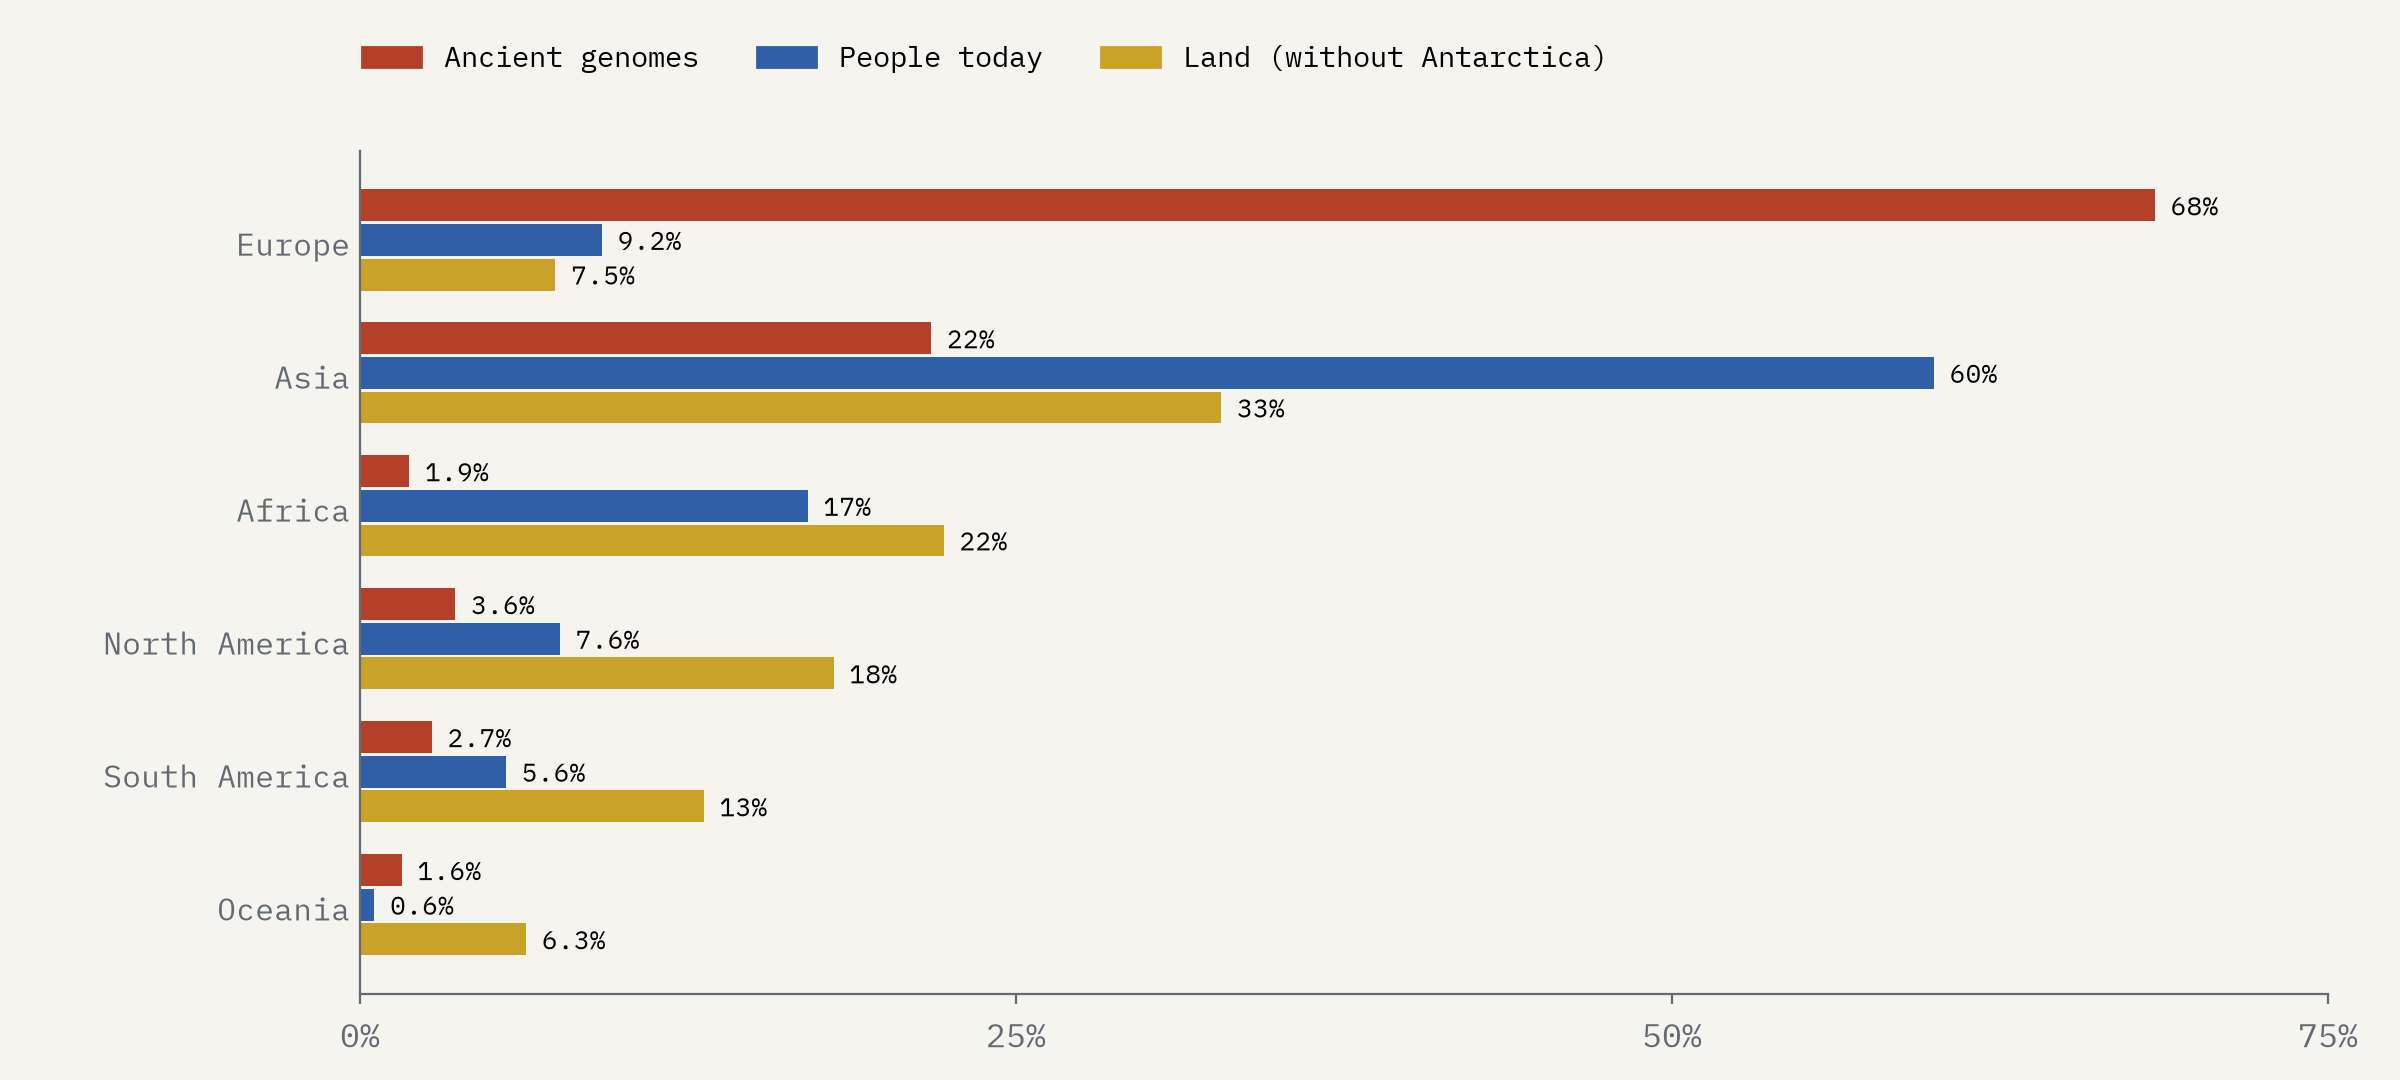
\includegraphics[width=\textwidth]{f_bias.png}
\caption{Share of ancient genomes, of present-day population and of land, by continent.}\label{fig:bias}\end{figure}

\subsection{The spread of farming}
Table~\ref{tab:neo} and Figure~\ref{fig:farmers} give the earliest Neolithic-labelled individual in each of 24 countries. The earliest is in Turkey (8750 BCE, Turkey\_PPNA). Among the other countries, dates fall later with distance from Çatalhöyük by 0.88 years per km (r = 0.75), equivalent to 1.13 km a year. By latitude band, the earliest Neolithic individual is from 6035 BCE at 45 to 50°N (Serbia), 5250 BCE at 50 to 55°N (Czechia) and 4110 BCE at 55 to 60°N (Denmark). The first Neolithic individual in Ireland is 4,954 years later than the first in Turkey.

\begin{table}[tbp]\centering\footnotesize\caption{Earliest individual labelled Neolithic per country (countries with at least three), with distance of its site from Çatalhöyük.}\label{tab:neo}\begin{tabular}{lrrlr}\toprule Country & Neolithic individuals & Earliest & Group & km\\\midrule
Turkey & 175 & 8750 BCE & Turkey\_PPNA & 794\\
Greece & 14 & 6366 BCE & Greece\_North\_N & 1,054\\
Serbia & 19 & 6143 BCE & Serbia\_EMN & 1,184\\
Italy & 40 & 6031 BCE & Italy\_Abruzzo\_N & 1,711\\
Romania & 19 & 6021 BCE & Romania\_EN\_Starcevo & 943\\
Hungary & 186 & 5990 BCE & Hungary\_EN\_LBK\_DVK & 1,524\\
Bulgaria & 22 & 5950 BCE & Bulgaria\_Yabalkovo\_N & 797\\
Croatia & 33 & 5913 BCE & Croatia\_N\_Cardial & 1,512\\
Austria & 88 & 5578 BCE & Austria\_N\_LBK & 1,792\\
France & 187 & 5413 BCE & France\_EN & 2,230\\
Spain & 63 & 5395 BCE & Spain\_EN & 2,671\\
Portugal & 22 & 5352 BCE & Portugal\_EN\_Cardial & 3,556\\
Czechia & 41 & 5250 BCE & Czechia\_EN\_LBK & 2,075\\
Germany & 157 & 5249 BCE & Germany\_StuttgartMuhlhausen2\_EN & 2,265\\
Slovakia & 57 & 5150 BCE & Slovakia\_N\_LBK & 1,677\\
Poland & 52 & 4441 BCE & Poland\_N\_LLBK\_LLengyel & 2,001\\
Switzerland & 50 & 4405 BCE & Switzerland\_LN & 2,331\\
Channel Islands & 6 & 4141 BCE & ChannelIslands\_MN & 3,098\\
Denmark & 58 & 4110 BCE & Denmark\_EN\_N\_TRB & 2,548\\
United Kingdom & 113 & 3981 BCE & England\_EN\_Megalithic & 3,120\\
Ireland & 50 & 3796 BCE & Ireland\_EN & 3,629\\
Sweden & 116 & 3796 BCE & Sweden\_MN & 2,883\\
Netherlands & 5 & 3700 BCE & Netherlands\_MN & 2,652\\
Belgium & 18 & 3203 BCE & Belgium\_N & 2,595\\
\bottomrule\end{tabular}\end{table}

\begin{figure}[tbp]\centering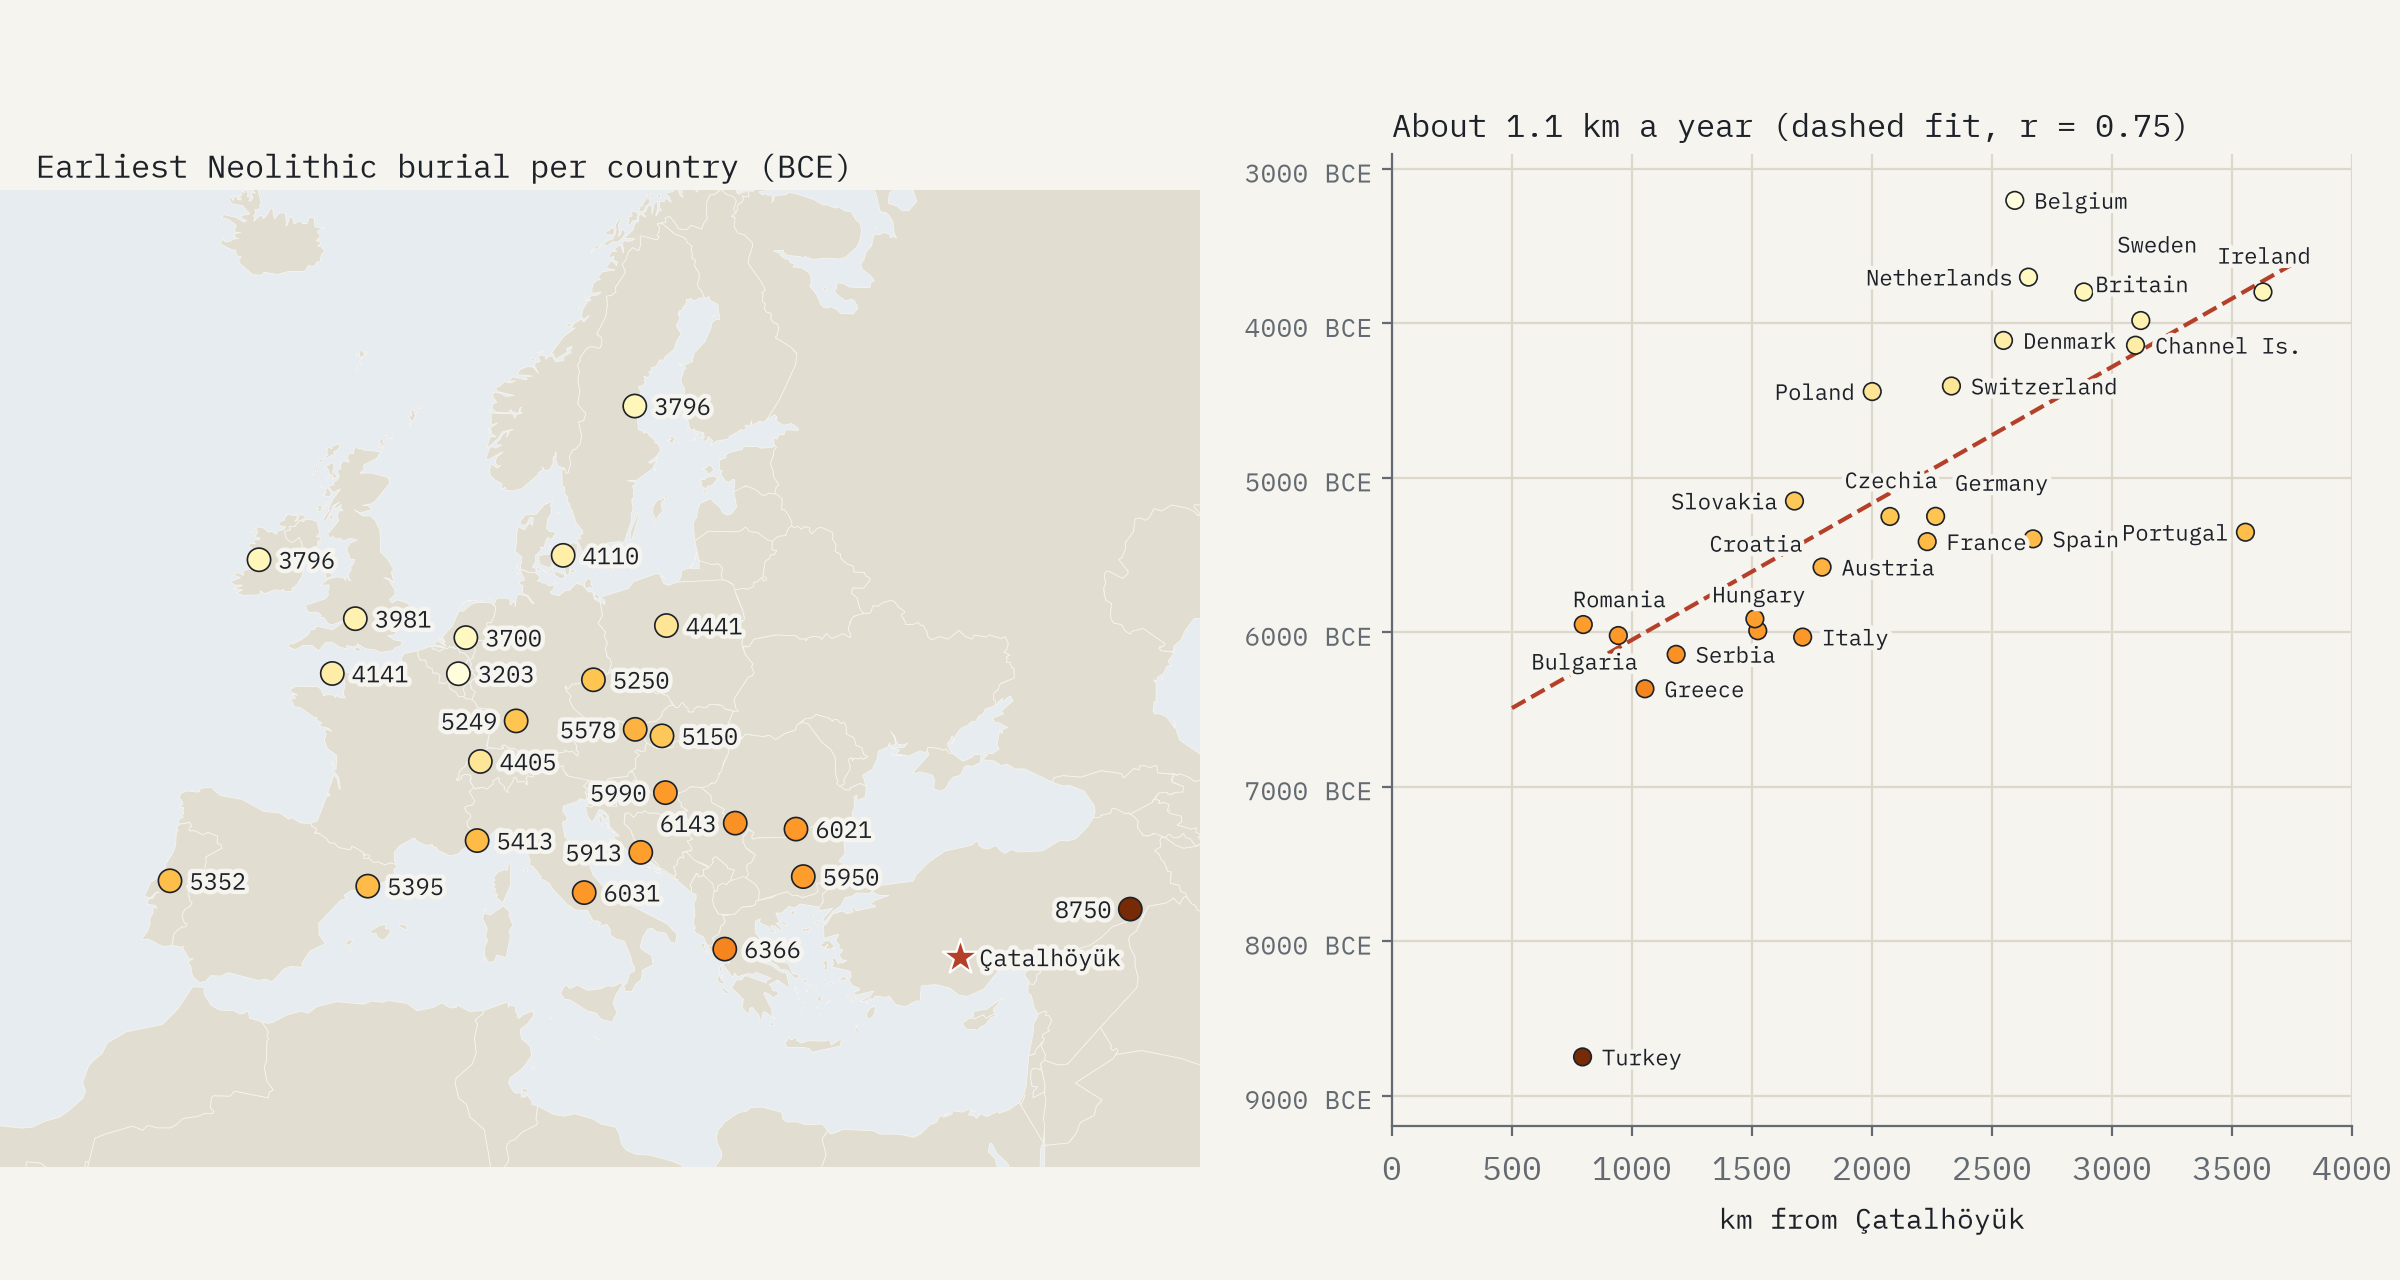
\includegraphics[width=\textwidth]{f_farmers.png}
\caption{Left: the earliest individual labelled Neolithic in each country (BCE). Right: its date against distance from Çatalhöyük, with the least squares line fitted without Turkey.}\label{fig:farmers}\end{figure}

\subsection{Y lines and the third millennium BCE}
Men labelled Yamnaya mostly carry R1b (128 of 163, 78.5\%); men labelled Corded Ware carry R1a (50.0\%) or R1b (41.3\%); men labelled Bell Beaker carry R1b (108 of 114). Among Neolithic men in Europe, 8.7\% carry R1b or R1a, 44.6\% I2 and 25.8\% G2. Within a Europe box (12°W to 45°E, 34 to 72°N), 7.9\% of 761 men dated 5000 to 3000 BCE carry R1b or R1a, against 65.0\% of 639 dated 2500 to 1500 BCE (Figure~\ref{fig:europe}).

In Britain (Figure~\ref{fig:britain}) none of the 76 men dated before 2500 BCE carries R1b or R1a; 71 carry I2. From 2500 to 1500 BCE, 50 of 56 carry R1b. The earliest R1b man is I3071 (England\_BellBeaker-ohighEEF, 2468-2294 calBCE (3900±30 BP, SUERC-32210)). R1b remains at 91.1\% in the Iron Age (800 BCE to 43 CE), and from 400 to 1066 CE I1 rises to 30.1\%, a clade carried by 35.2\% of Scandinavian men from 1 to 1000 CE. In the other three regions (Figure~\ref{fig:regions}) the share of R1b and R1a rises from 2.0\% (Iberia), 3.3\% (Scandinavia) and 4.8\% (central Europe) before 3000 BCE to 80.0\%, 51.1\% and 82.0\% from 2500 to 1500 BCE. In all four regions the first 500 year bin with at least five men in which at least half carry R1b or R1a is 2500 to 2000 BCE. The few earlier R1b men in central Europe (10 before 3000 BCE) are a reminder that R1b is an old clade with branches unrelated to the steppe.

\begin{figure}[tbp]\centering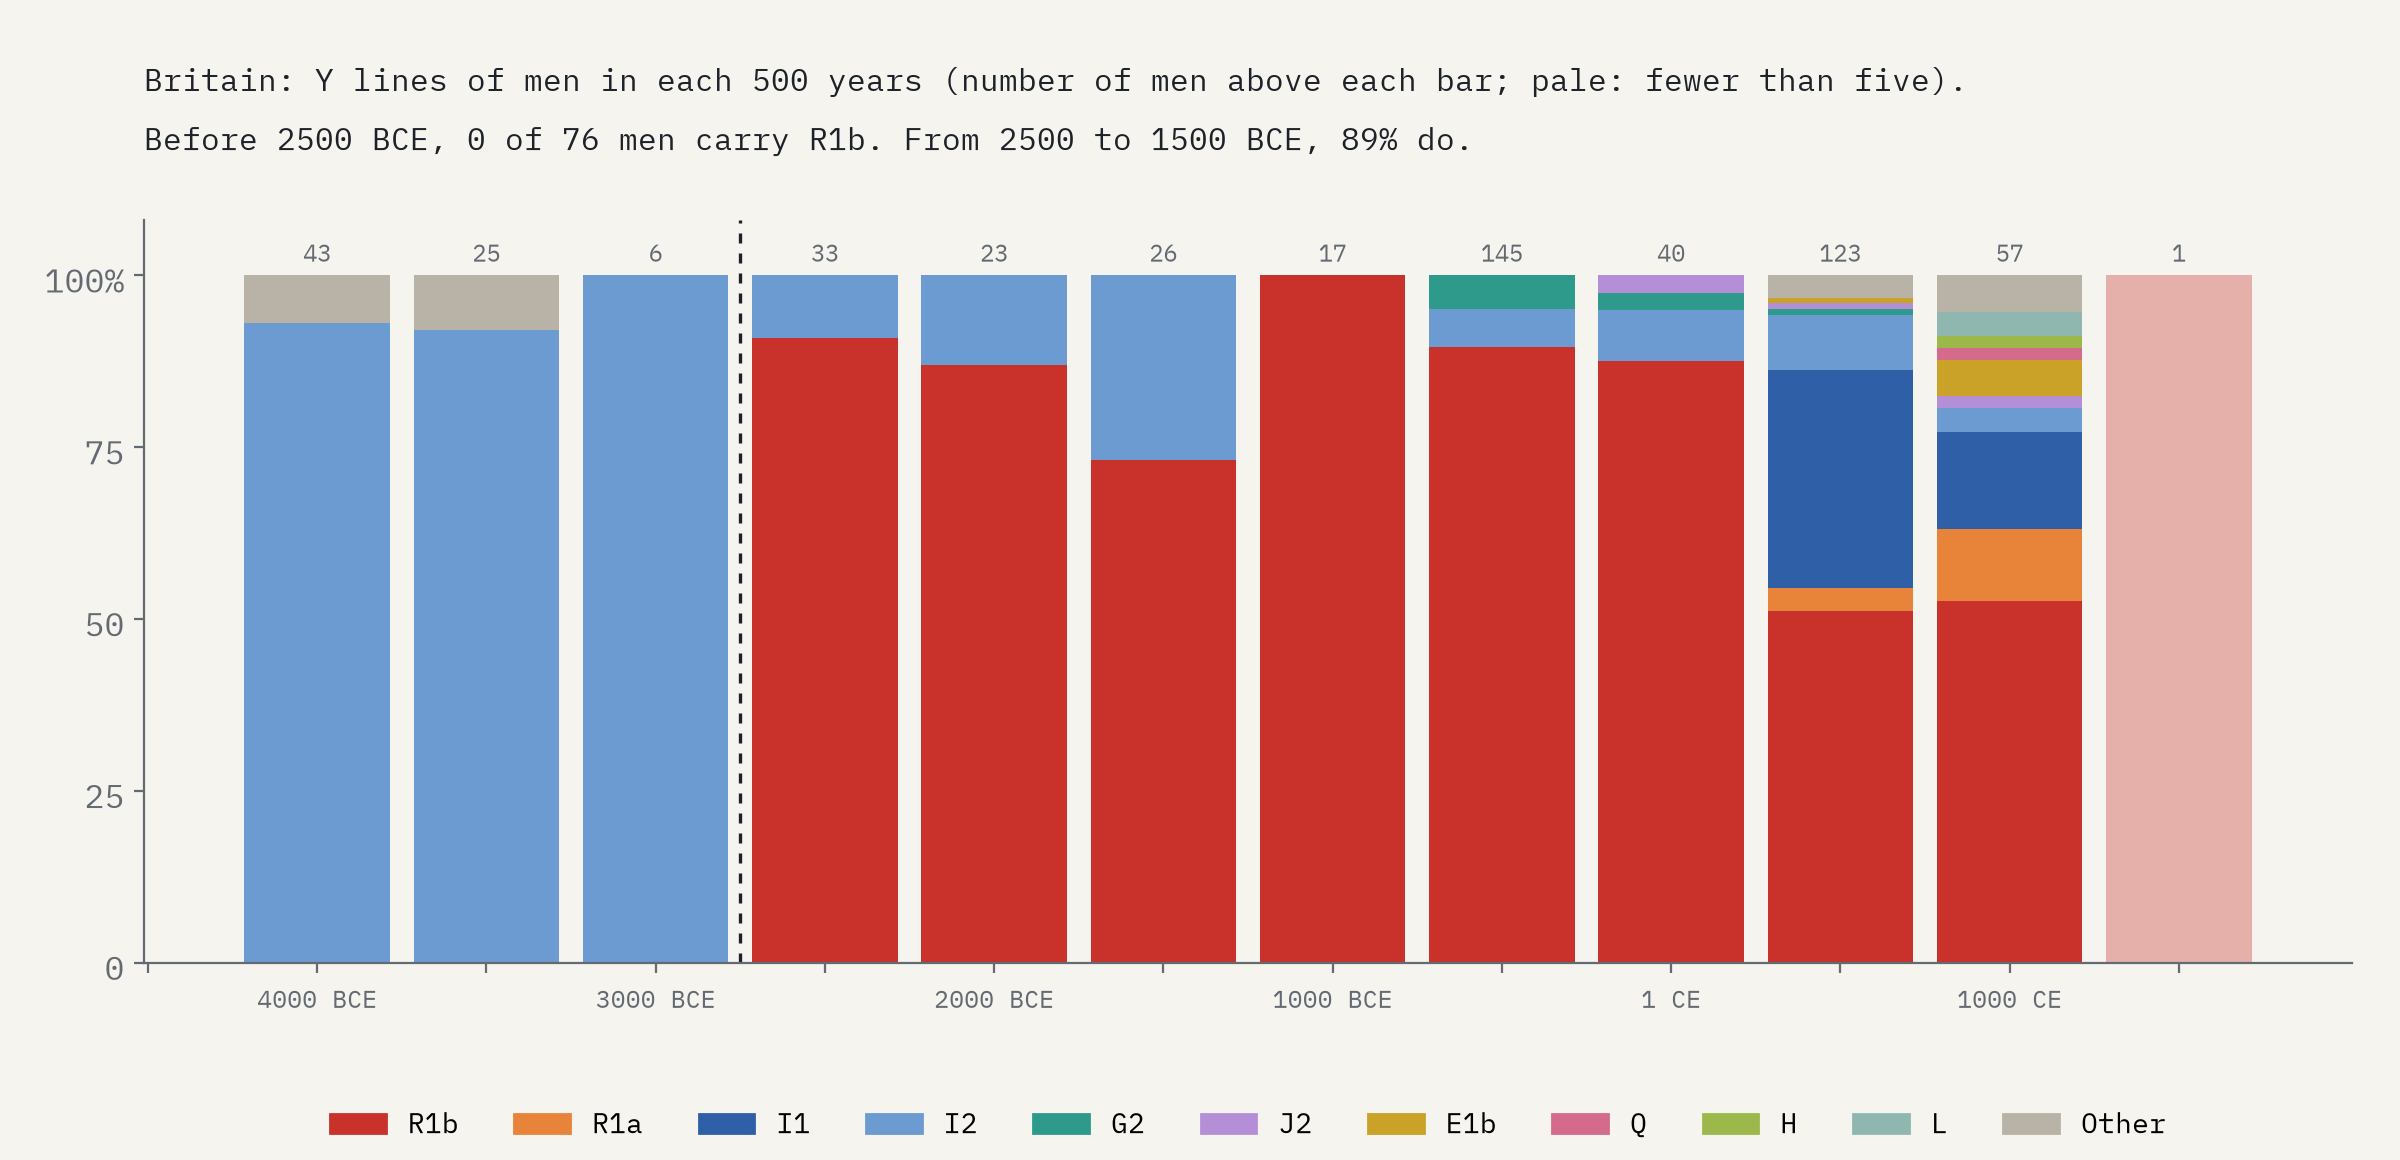
\includegraphics[width=\textwidth]{f_britain.png}
\caption{Y haplogroups of men in Britain per 500 years. Numbers above bars are men with a resolved call; pale bars have fewer than five. Dashed line: 2500 BCE.}\label{fig:britain}\end{figure}

\begin{figure}[tbp]\centering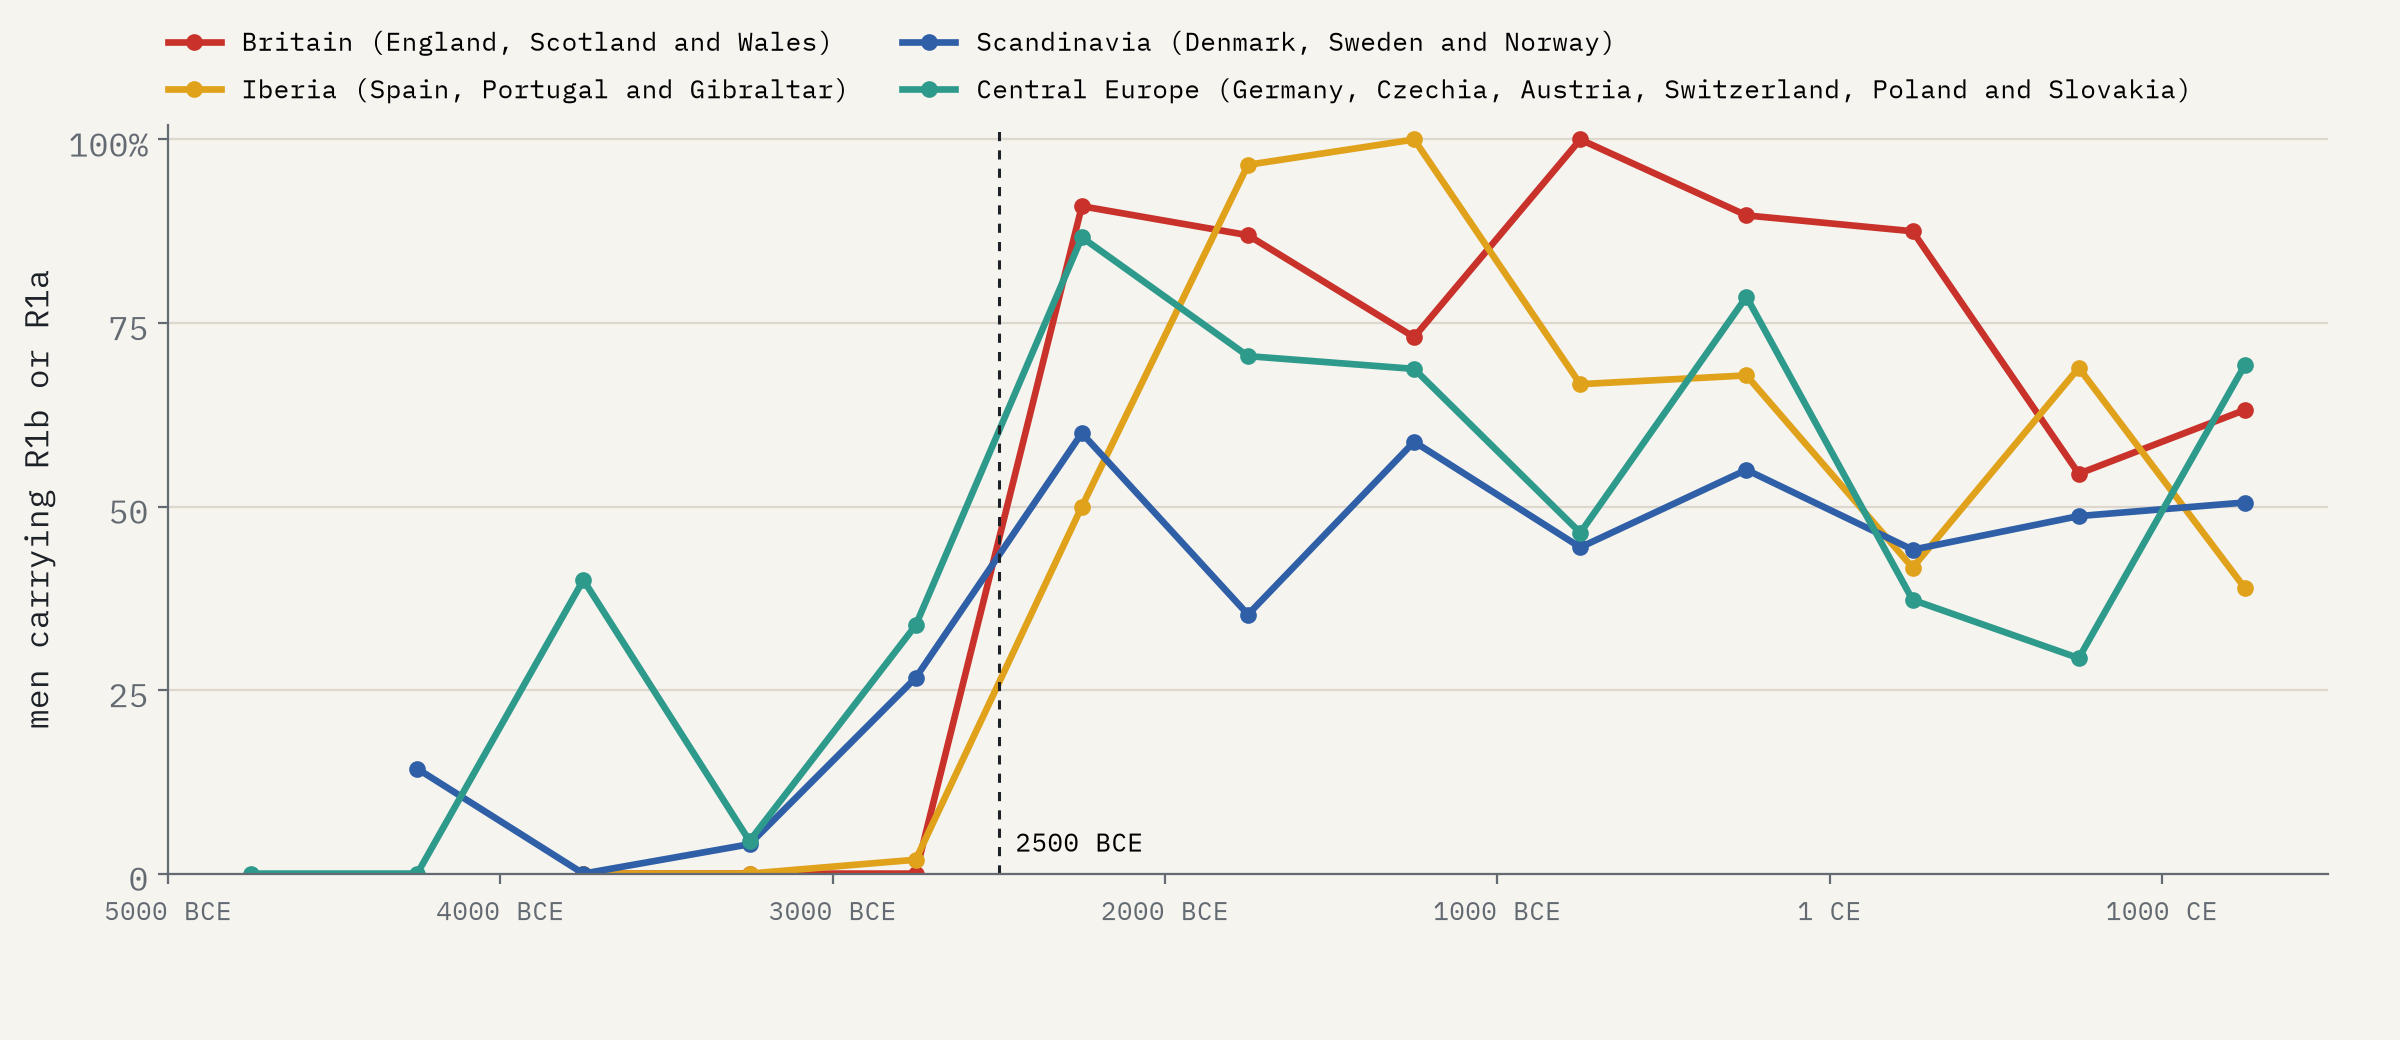
\includegraphics[width=\textwidth]{f_regions.png}
\caption{Share of men carrying R1b or R1a per 500 years in four regions (bins with at least five men).}\label{fig:regions}\end{figure}

\begin{figure}[tbp]\centering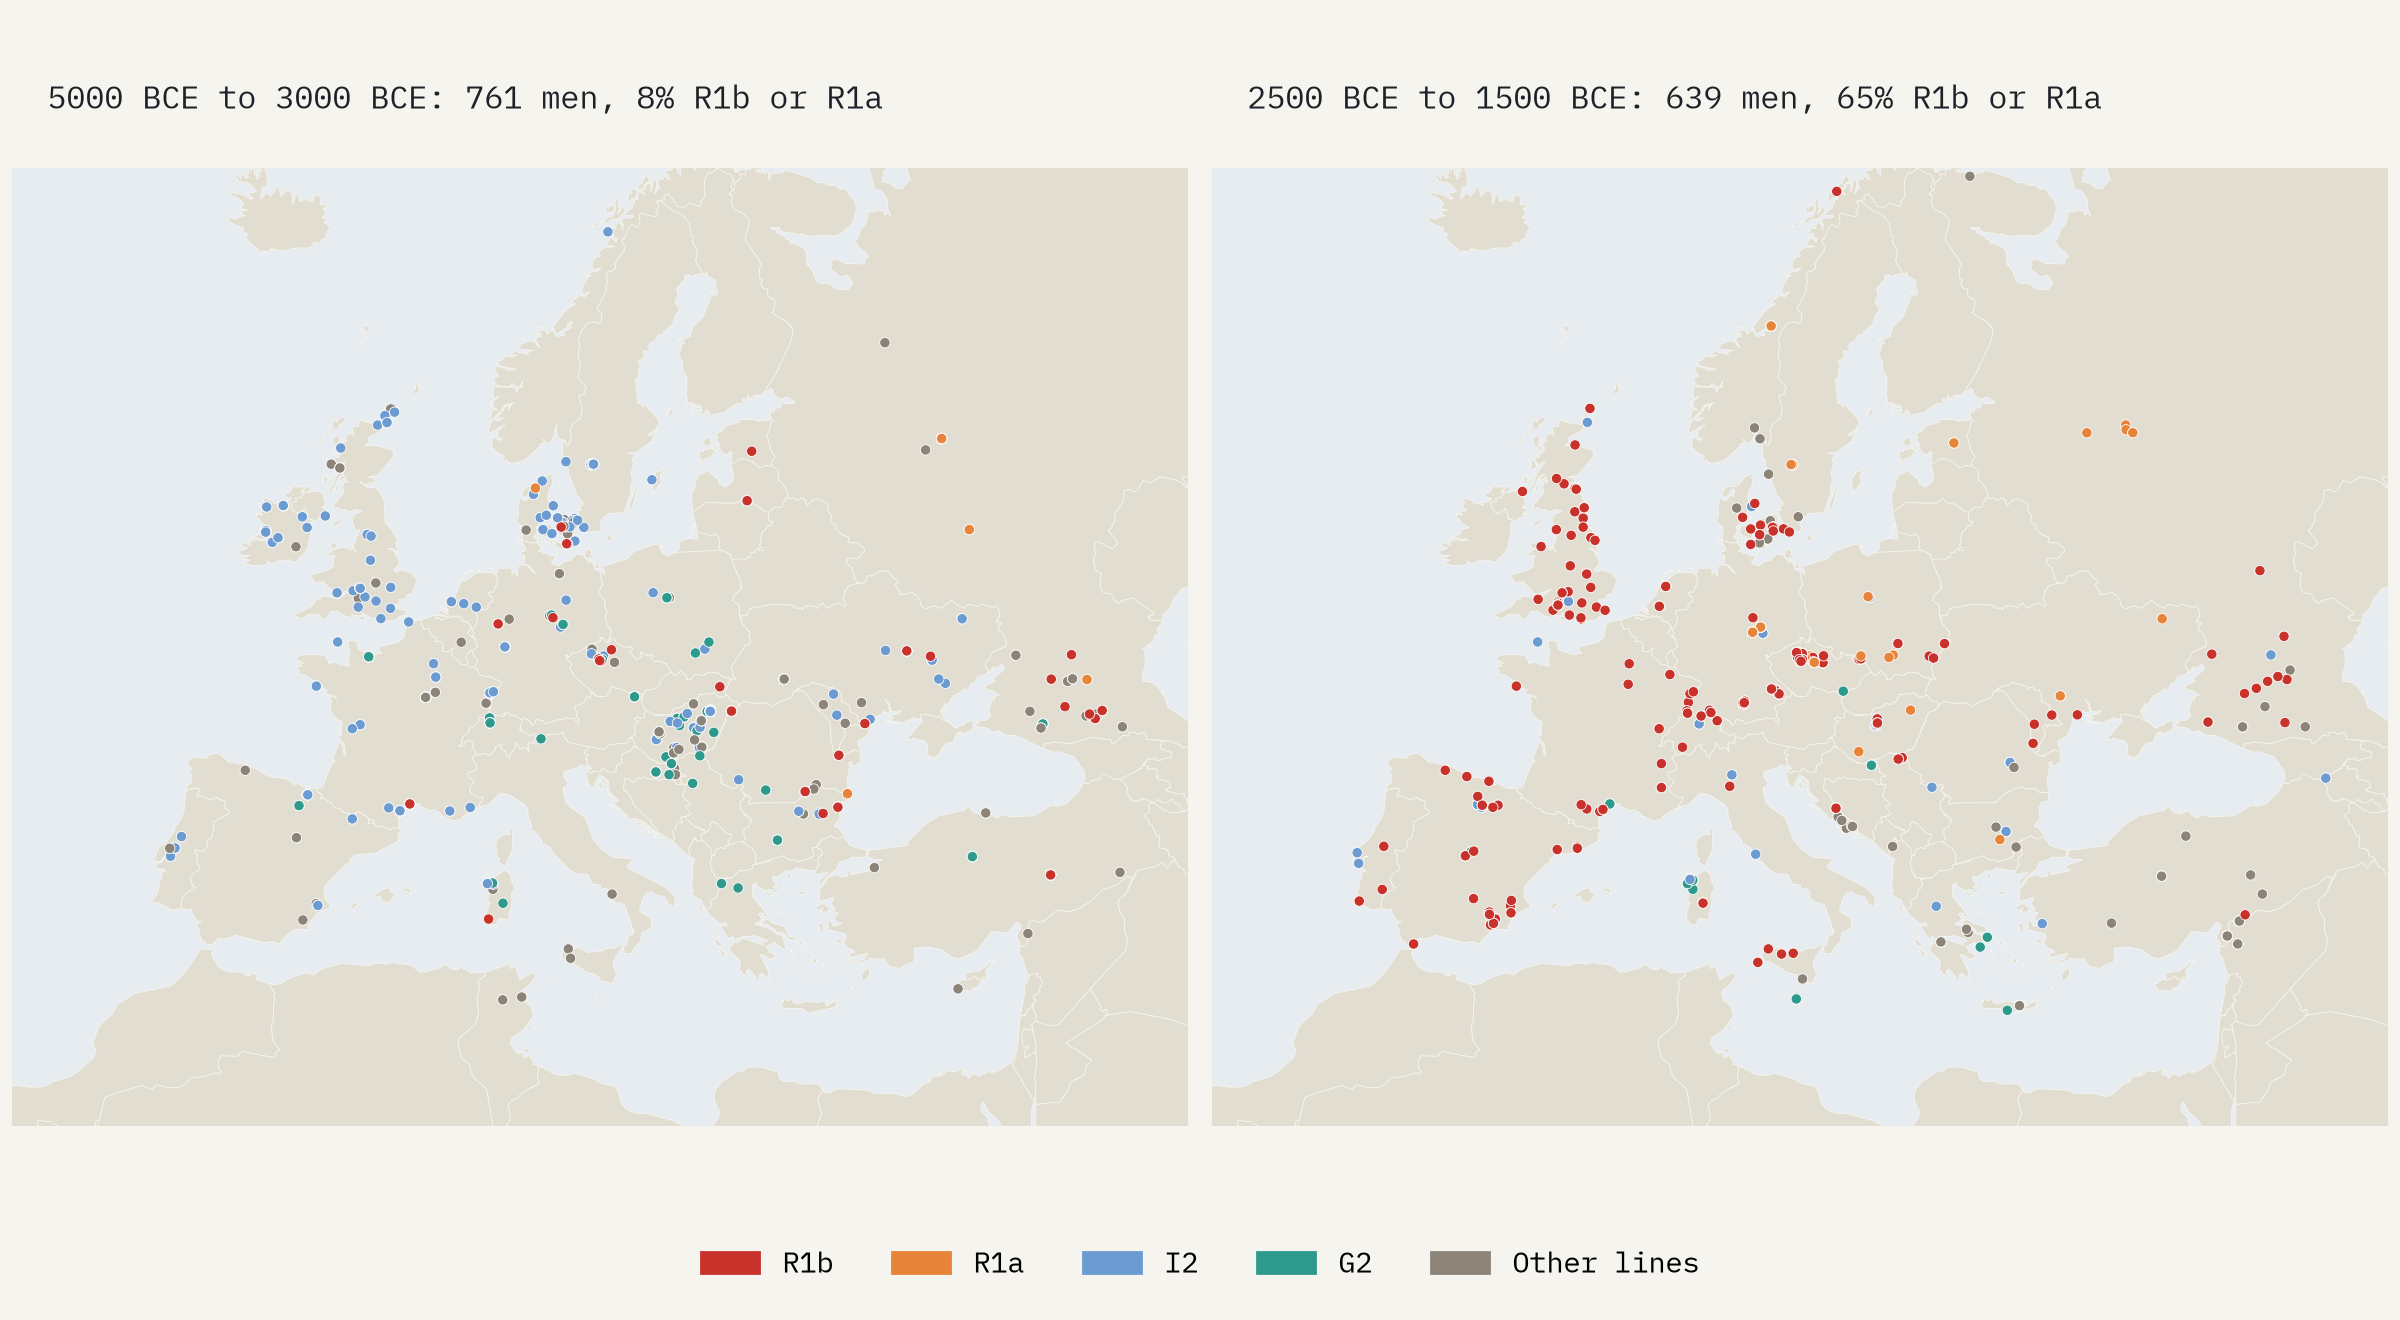
\includegraphics[width=\textwidth]{f_europe_y.png}
\caption{Men with a resolved Y haplogroup in Europe, 5000 to 3000 BCE (left) and 2500 to 1500 BCE (right).}\label{fig:europe}\end{figure}

\section{Limitations}
First, the archive reflects where research has been done, not where people lived, and every share here inherits that bias. Second, dates are the archive's means, some contextual and broad, and places are burial sites, sometimes given only to county level. Third, culture labels come from the archive's group names, which follow each study's own conventions; they are a convenience, not a classification. Fourth, the earliest sampled Neolithic burial in a country is a lower bound on the arrival of farming that depends on what has been dated and sequenced. Fifth, a Y haplogroup is one line of descent among thousands and is a proxy for ancestry, not ancestry itself: a change in Y lines can follow from differences in the number of sons men had, and genome-wide studies are needed to measure population change. Sixth, the quality filter follows the archive's own assessment; some well known individuals (Kennewick Man, the Anzick child) are graded Questionable and so are excluded.

\section{Conclusion}
The AADR now places more than sixteen thousand ancient people in time and space, most of them from the last five thousand years and most of them from Europe. Read simply, its annotations reproduce two central findings of archaeogenetics: a stepwise spread of Neolithic burials away from Anatolia at about a kilometre a year, and an abrupt change in male lines across western and central Europe around 2500 BCE, nowhere sharper than in Britain. They also show how unevenly the human past has been sampled.

\section*{Data and code availability}
The interactive map is at \url{https://maps.tristanhotham.com/ancient-dna/}. Data and code are at \url{https://github.com/Tristan-Hotham/ancient-dna} and archived with this paper at https://doi.org/10.5281/zenodo.23872993. Derived data are released under CC BY 4.0 and code under the MIT licence. The AADR is released under CC0 1.0 and should be cited as \citet{aadr,aadrpaper}; each genome should be credited to its original publication.

\section*{AI statement}
I wrote the text, with drafting and editing assistance from Claude (Anthropic), which also helped prepare the analysis code. I reviewed and checked all text and results.

\begin{thebibliography}{9}
\bibitem[Mallick et al.(2026)]{aadr} Mallick, S., Micco, A., Mah, M., Ringbauer, H., Lazaridis, I., Olalde, I., Patterson, N. and Reich, D. The Allen Ancient DNA Resource (AADR), version v66.p1. Harvard Dataverse. CC0 1.0. \url{https://doi.org/10.7910/DVN/FFIDCW}
\bibitem[Mallick et al.(2024)]{aadrpaper} Mallick, S. et al. (2024) The Allen Ancient DNA Resource (AADR) a curated compendium of ancient human genomes. Scientific Data 11, 182. \url{https://doi.org/10.1038/s41597-024-03031-7}
\bibitem[Natural Earth(2026)]{naturalearth} Natural Earth (2026) Admin 0 countries, land and populated places, 1:50m and 1:10m. Public domain. \url{https://www.naturalearthdata.com/}
\end{thebibliography}
\end{document}
